\chapter{Revisão Bibliográfica}      \label{Revisao Bibliografica}



\section{Nanofotônica}

Parágrafo.

\section{Dispositivos Fotônicos}

Parágrafo.

\subsection{Princípio de Funcionamento}

Parágrafo.

\subsection{Resposta em Frequência}

Parágrafo.


\section{Embasamento Teórico}      \label{Embasamento Teorico}

\subsection{Teoria de Grupos}

Parágrafo.


\subsection{Teoria de Modos Acoplados}

Parágrafo.


\section{COMSOL}

\subsection{Aspectos Gerais}


\subsection{Modelando Dispositivos Nanofotônicos}      \label{Modelando COMSOL}

\subsection{Malha}

\subsection{Estudo no Domínio da Frequência}

\subsection{Simulação}


\section{Machine Learning}

Parágrafo.

\subsection{Redes Neurais Artificiais}

Parágrafo.


\subsection{Fundamentos Biológicos}

Motivação: neurônio biológico.

\subsection{Neurônio Artificial}

\begin{figure}[H]
    \centering
    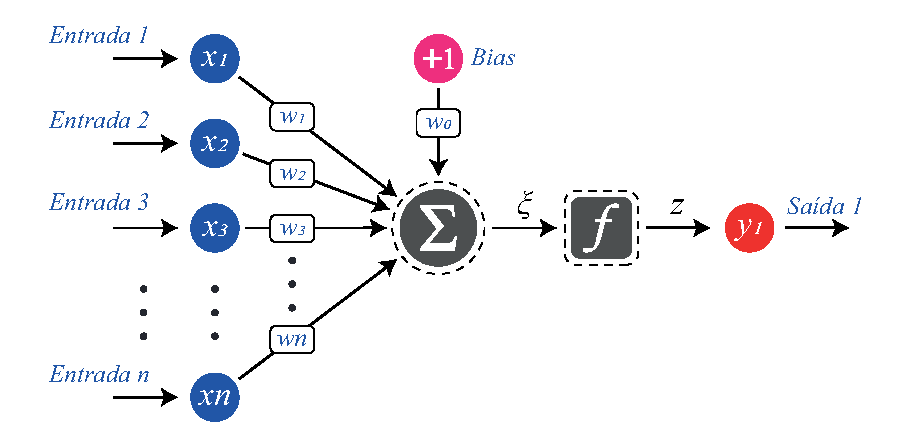
\includegraphics{04-Figuras/ArtificialNeuronModel.eps}
    \caption{Arquitetura de um neurônio artificial.} \par
    Fonte: do Autor.
    \label{figura: ArtificialNeuronModel}
\end{figure}




\subsection{Função de Ativação}

Parágrafo.


\subsection{Algorítmo de Aprendizagem}

Parágrafo.


\subsection{Algorítmo Backpropagation}

Parágrafo.